\documentclass{../../note}

\usepackage{amsthm}
\usepackage{pgfplots}
\pgfplotsset{compat=1.18}
\usepackage{xcolor}
\usepackage{tikz}
\usetikzlibrary{shapes,arrows,positioning,fit,calc,matrix,decorations.pathreplacing}
\usepackage{algorithm}
\usepackage{algpseudocode}
\usepackage{listings}
\usepackage{booktabs}
\usepackage{array}
\usepackage{enumitem}

\lstset{
  basicstyle=\ttfamily\small,
  keywordstyle=\color{blue},
  commentstyle=\color{green!60!black},
  stringstyle=\color{purple},
  numbers=left,
  numberstyle=\tiny,
  numbersep=5pt,
  breaklines=true,
  frame=single,
}

\title{HUFE 数据结构模拟试卷 B}
\author{isomo}
\setlength{\parindent}{0em}

\begin{document}

\fontsize{12pt}{14.4pt}\selectfont
\maketitle

本卷依据最新考纲与课程时间安排整理，适合作为第二套综合训练题，强化树、图、查找和排序应用。

\section*{一、填空题（10空，每空2分，共20分）}

\begin{enumerate}[itemsep=0.8em]
\item 数据结构从逻辑上通常分为\underline{\hspace{2cm}}结构和\underline{\hspace{2cm}}结构。
\item 设顺序表中有 $n$ 个元素，在第 $i$ 个位置插入一个新元素，最坏情况下需要移动\underline{\hspace{2cm}}个元素。
\item 链队列进行出队操作时，一般在\underline{\hspace{2cm}}端删除元素，在\underline{\hspace{2cm}}端插入元素。
\item 若一棵满二叉树的深度为 $k$，则该树共有\underline{\hspace{2cm}}个结点。
\item 设一个有向图有 $n$ 个顶点，则其完全有向图最多有\underline{\hspace{2cm}}条有向边。
\item 图的广度优先遍历在实现思想上类似于树的\underline{\hspace{2cm}}遍历。
\item 哈希表的装填因子定义为\underline{\hspace{2cm}}。
\item 快速排序的平均时间复杂度为\underline{\hspace{2cm}}。
\item 若某线性表主要进行随机访问操作，通常应采用\underline{\hspace{2cm}}存储结构。
\item 对一个关键字序列进行排序后，相同关键字的相对次序不变，这一性质称为排序算法的\underline{\hspace{2cm}}。
\end{enumerate}

\section*{二、单项选择题（10题，每题2分，共20分）}

\begin{enumerate}[itemsep=0.8em]
\item 下列说法中错误的是（\hspace{0.8cm}）。

A．线性表中每个结点最多只有一个直接前驱和一个直接后继
\quad B．树中每个结点都只有一个直接前驱
\quad C．图中任意两个顶点之间都必须有边
\quad D．二叉树是树的一种特殊形式

\item 对于一个带头结点的单链表，在结点 $p$ 之后插入结点 $s$ 的正确操作是（\hspace{0.8cm}）。

A．$s\to next=p;\ p\to next=s;$
\quad B．$s\to next=p\to next;\ p\to next=s;$
\quad C．$p\to next=s;\ s\to next=p\to next;$
\quad D．$p=s;\ s\to next=NULL;$

\item 一个栈的输入序列为 $1,2,3,4$，则可能的输出序列是（\hspace{0.8cm}）。

A．3,4,1,2 \quad B．2,4,3,1 \quad C．4,2,3,1 \quad D．3,1,4,2

\item 设一棵二叉树共有 $n$ 个结点，则该二叉树中空指针域的个数为（\hspace{0.8cm}）。

A．$n-1$ \quad B．$n$ \quad C．$n+1$ \quad D．$2n$

\item 若无向连通图有 $n$ 个顶点，则其最小生成树一定包含（\hspace{0.8cm}）。

A．$n$ 条边 \quad B．$n-1$ 条边 \quad C．$n+1$ 条边 \quad D．不确定

\item 对一组记录按关键字进行排序，若要求每趟可以确定一个元素最终位置，则最适合的方法是（\hspace{0.8cm}）。

A．简单选择排序 \quad B．归并排序 \quad C．基数排序 \quad D．折半插入排序

\item 对于二叉排序树，下列叙述正确的是（\hspace{0.8cm}）。

A．左子树上所有结点值都小于根结点值
\quad B．左右子树高度必须相等
\quad C．只要有中序序列就能唯一确定二叉排序树
\quad D．删除结点时只能删除叶子结点

\item 若采用邻接矩阵存储一个有 100 个顶点的稀疏图，则其主要缺点是（\hspace{0.8cm}）。

A．不便于判断两顶点是否相邻
\quad B．不便于进行 DFS
\quad C．浪费存储空间
\quad D．无法表示带权图

\item 下列查找方法中，平均查找效率与结点分布情况关系最密切的是（\hspace{0.8cm}）。

A．顺序查找 \quad B．折半查找 \quad C．哈希查找 \quad D．二叉排序树查找

\item 在下列排序方法中，不稳定的是（\hspace{0.8cm}）。

A．冒泡排序 \quad B．直接插入排序 \quad C．归并排序 \quad D．快速排序
\end{enumerate}

\section*{三、判断题（10题，每题1分，共10分）}

\begin{enumerate}[itemsep=0.6em]
\item 数组和广义表都属于线性结构。 （\hspace{0.8cm}）
\item 在链式存储结构下，插入和删除元素时通常不需要移动大量元素。 （\hspace{0.8cm}）
\item 循环队列可以避免顺序队列中的“假溢出”问题。 （\hspace{0.8cm}）
\item 完全二叉树一定是满二叉树。 （\hspace{0.8cm}）
\item 一个连通图的生成树可能不唯一。 （\hspace{0.8cm}）
\item Dijkstra 算法适用于求带负权边图的最短路径。 （\hspace{0.8cm}）
\item 哈希查找在任何情况下时间复杂度都为 $O(1)$。 （\hspace{0.8cm}）
\item 折半查找既适用于顺序表，也适用于单链表。 （\hspace{0.8cm}）
\item 堆排序和快速排序都属于交换排序。 （\hspace{0.8cm}）
\item 归并排序需要额外的辅助空间。 （\hspace{0.8cm}）
\end{enumerate}

\section*{四、简答题（4题，每题5分，共20分）}

\begin{enumerate}[itemsep=1em]
\item 简述顺序栈与链栈各自的优缺点。
\item 什么是完全二叉树？什么是满二叉树？两者有何联系与区别？
\item 简述邻接矩阵和邻接表在空间开销以及求顶点邻接点方面的差异。
\item 什么是哈希冲突？请写出两种常见的冲突处理方法，并说明其基本思想。
\end{enumerate}

\section*{五、综合应用题（3题，每题10分，共30分）}

\begin{enumerate}[itemsep=1.2em]
\item 已知关键字序列依次为 $45,24,53,12,37,93,50$，按该顺序构造二叉排序树。
\begin{enumerate}[label=(\arabic*)]
\item 画出构造后的二叉排序树；
\item 写出该树的中序遍历序列；
\item 若删除关键字 24，画出删除后的二叉排序树。
\end{enumerate}

\item 已知有向带权图如下图所示，以顶点 $A$ 为源点。
\begin{enumerate}[label=(\arabic*)]
\item 写出从 $A$ 出发的一种深度优先遍历序列；
\item 用 Dijkstra 算法求从 $A$ 到各顶点的最短路径长度；
\item 写出从 $A$ 到 $E$ 的最短路径。
\end{enumerate}

\begin{center}
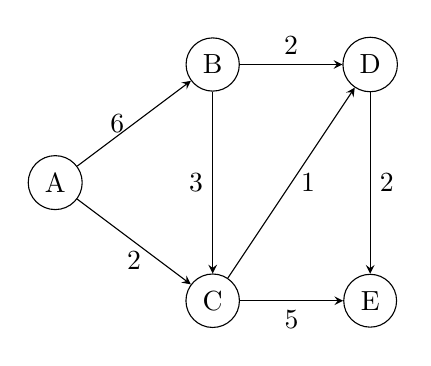
\begin{tikzpicture}[>=stealth]
  \node[circle,draw] (A) at (0,1.5) {A};
  \node[circle,draw] (B) at (2,3) {B};
  \node[circle,draw] (C) at (2,0) {C};
  \node[circle,draw] (D) at (4,3) {D};
  \node[circle,draw] (E) at (4,0) {E};

  \draw[->] (A) -- node[left] {6} (B);
  \draw[->] (A) -- node[below] {2} (C);
  \draw[->] (B) -- node[above] {2} (D);
  \draw[->] (B) -- node[left] {3} (C);
  \draw[->] (C) -- node[below] {5} (E);
  \draw[->] (C) -- node[right] {1} (D);
  \draw[->] (D) -- node[right] {2} (E);
\end{tikzpicture}
\end{center}

\item 给定待排序序列 $\{49,38,65,97,76,13,27,49\}$。
\begin{enumerate}[label=(\arabic*)]
\item 写出冒泡排序前两趟后的结果；
\item 写出简单选择排序第一趟和第二趟后的结果；
\item 比较冒泡排序和简单选择排序在比较次数、移动次数以及稳定性方面的特点。
\end{enumerate}
\end{enumerate}

\end{document}
